\chapter{Introduction}
% Following the PLoS guidelines, I will use sections, subsections, and paragraphs for my headings.
This thesis focuses on the human microbiome, its relation to human diseases, and techniques used in the analysis and exploration of data derived from it. During the course of my thesis, I conducted one study about nonalcoholic fatty liver disease, and investigated alternate weightings of a common microbiome analysis technique (UniFrac). Each of these topics is represented as a chapter of my thesis.

\section{The human microbiome}
Approximately half of the cells that make up the human body are bacterial \cite{sender2016revised}. Trillions of these bacteria live in the gut \cite{guarner2003gut}, and have a massive metabolic potential. For example, the gut microbiome has been shown to produce changes in hormone levels \cite{markle2013sex}, short chain fatty acid levels \cite{turnbaugh2008diet}, and ethanol levels \cite{krebs1970physiological}, to name a few. The human gut microbiome can also digest polysaccharides otherwise unusable by humans \cite{flint2008polysaccharide}.

This massive metabolic potential produces measurable physiological effects. Transplanting gut bacteria from obese mice to lean mice has been shown to allow lean mice to absorb more calories from the same amount of food, thereby becoming more obese \cite{turnbaugh2006obesity}. The microbiome can also affect behavior: Completely germ free mice exhibit more anxiety-like behaviors than specific pathogen free mice that contain a complex gut microbiome \cite{neufeld2011reduced}.

Study of the human microbiome opens up a host of possibilities for reducing the effects of disease and improving quality of life. However, until recently, a deep understanding of the human microbiome has been beyond the reach of available technology. For example, \textit{Escherichia coli} is a common model gut bacteria because it is easy to culture, however in reality this species makes up less than 1\% of the average human gut microbiome \cite{arumugam2011enterotypes}.

With the advent of next generation DNA and RNA sequencing, scientists can obtain a more comprehensive snapshot of the bacterial composition of the microbiome, what genes are present, and what proteins are produced \cite{di2013high}. We are in a phase of developing the experiments and accompanying statistical techniques to elucidate the exact mechanisms by which the human microbiome affects health and disease. Armed with a deeper understanding of how the microbiome works, we may be able to modulate the microbiome to improve quality of life.

\section{Exploring the human microbiome}
The advent of next generation DNA sequencing prompted the development of various experiments on sampling the human microbiome. Samples can be collected by swabbing the target body site or collecting excretions such as saliva or stool. Products such as DNA or RNA may be extracted from these samples as appropriate for the analysis.

A comparative study design involves an experimental group and a control group. The study subjects can be patients with disease and healthy controls \cite{macklaim2013comparative}, people who are susceptible and resistant to a condition \cite{theriot2014antibiotic}, or patients before and after a medical intervention \cite{graessler2013metagenomic}. The questions that scientists in this field want to answer are: Is the human microbiome driving or associated with the difference between the two groups? If so, what is the mechanism of action? There are also exploratory studies that try to determine the similarities in the microbiomes of specific body sites among patients with similar medical conditions.

Next generation sequencing experiments can deduce: Is there a significant difference in the microbiome between the control and the experimental groups? Is this difference due to different types of microbes present or the microbial genes present? Do separated groups exist in the data? Are the abundances of certain taxa or genes correlated with each other, or with patient metadata? Through metagenomic experiments and statistical analysis we can gather clues about the larger questions of the mechanism of action.

In this thesis, I have performed two experiments that can be done with microbiome next generation DNA sequencing data: gene tag abundance (Fig. ~\ref{16s_workflow}) and metagenomic sequencing (Fig. ~\ref{metagenomic_workflow}) \cite{riesenfeld2004metagenomics}. The tag used for gene tag abundance here is the conserved 16S rRNA gene, which is related to taxonomic identity \cite{gloor2010microbiome}.

\section{Illumina next generation sequencing}
The Illumina MiSeq and HiSeq are next generation sequencing platforms. The Illumina MiSeq machines yields up to 25 million paired end reads up to 300 nucleotides long. The Illumina HiSeq machines yield up to 4 billion paired end reads \cite{bentley2008accurate}. The general sequencing workflow is as follows:

\begin{enumerate}
\item DNA is amplified or fragmented to smaller pieces of approximately 1000 nucleotides or less
\item Adaptors are joined to the ends of the DNA
\item The DNA is denatured
\item The DNA is placed on a flow cell covered in oligonucleotides complimentary to the adaptor sequences, such that the DNA fragments are bound to the oligonucleotides
\item The DNA on the flow cell is replicated \textit{in situ} to form clusters of identical sequences
\item The DNA is denatured
\item Primers, nucleotides, DNA polymerase, and fluorescently labelled deoxyribonucleotide triphosphate terminators are added
\item A microscope can detect the fluorescently labelled nucleotide terminators for each added base on each cluster of identical sequences, allowing the DNA to be sequenced.
\item Fluorescent terminators are removed, exposing a 3'OH
\item Steps 7-9 are repeated until the desired number of cycles is complete.
\end{enumerate}

The Illumina sequencing technology is the industry standard for metagenomic studies \cite{bentley2008accurate}, and library preparation kits and protocols are available commercially. Roche 454 pyrosequencing \cite{margulies2005genome} and sequencing on the SOLiD platform \cite{shendure2005accurate} \cite{mckernan2009reagents} are other next generation sequencing options. The pyrosequencing platform has the advantage of longer reads, but yields higher error rates and is more expensive. SOLiD uses shorter read lengths and also has a higher error rate \cite{mardis2008next} \cite{shendure2008next}.

One unappreciated feature of Illumina and other next generation DNA sequencing technologies is that they deliver data as parts per machine limit, not a count of molecules in the sample \cite{fernandes2013anova} \cite{fernandes2014unifying} \cite{gloor2010microbiome} \cite{gloor2016compositional} \cite{gloor2016s}. Different Illumina machines are configured to yield different numbers of reads - the MiSeq machines yield millions of reads while the HiSeq machines yield billions \cite{caporaso2012ultra}. The total number of reads is not reflective of any property of the biological sample. As parts per machine limit, the read counts should be analyzed as compositional data \cite{aitchison1982statistical}.

\section{Gene tag abundance}
Historically, Koch’s postulates have been used to determine if a microbe is a disease-causing pathogen. Koch's postulates are:

\begin{enumerate}
\item The microbe must be present in all cases of the disease.
\item The microbe must not be present but non-pathogenic in other diseases.
\item If the microbe is isolated in pure culture, it can be used to induce the disease \cite{koch1891uber}.
\end{enumerate}

Fredricks et al. have created a modified set of postulates that takes DNA sequencing into account which can be applied to differentially abundant taxa detected by gene tag sequencing \cite{fredericks1996sequence}:

\begin{enumerate}
\item A nucleic acid sequence belonging to a putative pathogen should be present in most cases of an infectious disease. Microbial nucleic acids should be found preferentially in those organs or gross anatomic sites known to be diseased and not in those organs that lack pathology.
\item Fewer, or no, copy numbers of pathogen-associated nucleic acid sequences should occur in hosts or tissues without disease.
\item With resolution of disease (for example, with clinically effective treatment), the copy number of pathogen-associated nucleic acid sequences should decrease or become undetectable. With clinical relapse, the opposite should occur.
\item When sequence detection predates disease, or sequence copy number correlates with severity of disease or pathology, the sequence-disease association is more likely to be a causal relationship.
\item The nature of the microorganism inferred from the available sequence should be consistent with the known biological characteristics of that group of organisms. When phenotypes are predicted by sequence-based phylogenetic relationships, the meaningfulness of the sequence is enhanced.
\item Tissue-sequence correlates should be sought at the cellular level: efforts should be made to demonstrate specific in situ hybridization of microbial sequence to areas of tissue pathology and to visible microorganisms or to areas where microorganisms are presumed to be located.
\item These sequence-based forms of evidence for microbial causation should be reproducible.
\end{enumerate}

However, Koch’s postulates do not account for when the same bacteria can have a very different expression profile in health and disease, such as \textit{Lactobacillus iners} in bacterial vaginosis \cite{macklaim2013comparative}. Gene tag abundance takes us beyond Koch's postulates to the effect of consortia of microbiota.

Gene tag abundance experiments provide an estimate of the proportion of different bacterial taxa in the sample. This can be used to answer questions such as:

\textit{What bacterial taxa make up the microbial community?}
Scientists often want to characterize microbiomes for certain conditions. Perhaps body site microbiomes of people with a condition share certain bacterial taxa or microbial properties. The idea is that characterizing what this core microbiome is can lead to insight on core functions and how they can be altered when the core microbiome is disrupted.

For example, the core gut microbiome was described by one group to have three enterotypes \cite{arumugam2011enterotypes}. The enterotype structure would have been very useful for measuring the association of certain enterotypes with conditions, and for observing how gut microbiomes transition across enterotypes. However, when another group studied a diverse population including non-Western people, the enterotypes did not hold \cite{yatsunenko2012human}. A second group showed that these enterotypes were artifacts induced by the analysis methods that depended on the abundance of the predominant taxa \cite{gorvitovskaia2016interpreting}. The gut microbiome is highly diverse between individuals, and the enterotype model does not capture this diversity.

An example of a successfully characterized body site is the vaginal microbiome. The vaginal microbiome is known to be \textit{Lactobacillus} dominated, except in bacterial vaginosis \cite{hummelen2010deep} or anaerobic vaginitis \cite{donders2002definition}, where the microbiome is much more diverse. The bacterial composition of vaginal microbiomes in bacterial vaginosis have high variation, however their expression profiles are similar, allowing for functional characterization in the absence of taxonomic characterization \cite{macklaim2013comparative}.

\textit{Are there any differentially abundant taxa between conditions?}
Some theories of disease progression include the involvement of bacteria as pathogens. Others involve bacteria as probiotics, preventing disease progression.

For example, in atopic dermatitis, a flare-up is defined as an acute exacerbation of disease despite standard treatment. Flare-ups are associated with a significant increase in the proportion of \textit{Staphylococcus aureus} on the skin \cite{kong2012temporal}. However, the exact mechanisms by which \textit{Staphylococcus aureus} causes atopic dermatitis are unknown.

Bacteria have also been used for therapy in the treatment of \textit{Clostridium difficile}. Stool transplants have been found to be more effective than the vancomycin antibiotic \cite{van2013duodenal}. Work is being done to standardize treatments: In one study, 33 microbes cultured from a healthy donor were used to successfully treat symptoms, with no recurrence throughout the 6 month follow up period \cite{petrof2013stool}.

\textit{Do samples from different conditions cluster together?}
Beta diversity distance similarities between microbiomes can be examined for distinct sites or conditions. This is often done with distance or dissimilarity metrics, such as the UniFrac distance and the Bray Curtis dissimilarity.

Sometimes when the data is plotted, there appears to be separation between groups, even if specific taxa are not differentially abundant. One example of this is a study on discordant gut microbiomes between twins in Malawi where one twin has a protein-deficient form of malnourishment called kwashiorkor, and the other is healthy \cite{smith2013gut}. In this case the microbiomes were seen to diverge the most during treatment with ready-to-use therapeutic food.

\subsection{16S rRNA gene sequencing experiment}
The gene tag chosen for analysis throughout this thesis is the gene for the 16S subunit of ribosomal RNA. The 16S rRNA gene is present in all known bacteria and has regions of variability interspersed with regions of high conservation. This allows primers to be made to match the conserved regions, such that the variable regions can be amplified, sequenced, and used to infer taxonomy. Entire databases exist specifically to match the 16S rRNA gene with taxonomy, such as SILVA \cite{quast2013silva}, the Ribosomal Database Project \cite{cole2009ribosomal}, and Greengenes \cite{desantis2006greengenes}.

Specifically, this work uses the 16S rRNA gene primers from the Earth Microbiome Project protocol \cite{gilbert2014earth}, which amplify the V4 variable region of the 16S rRNA gene. This region was identified by PrimerProspector to be nearly universal to archaea and bacteria \cite{walters2011primerprospector}.

\subsection{Operational Taxonomic Units}
Unlike more distinct species, such as mammalian species, bacterial species are not well defined. Bacterial genomes are highly variable, and regions used to identify bacteria vary in a continuum rather than clusters of similar sequences.

Historically bacteria that have 97\% identity in a variable region are considered to be the same taxa. The 97\% cutoff was arbitrarily chosen to best map sequence data to bacterial classifications. This threshold maximizes the grouping of bacteria classified as the same species while minimizing the grouping of bacteria classified as different species. Before sequencing bacterial classification was often done by appearance or by metabolic products, so there are examples where bacteria classified in the same species are actually genetically very different, or bacteria classified in different genera are genetically very similar \cite{ciccarelli2006toward}.

However, it is difficult to determine how a batch of sequences should be partitioned into groups of 97\% identity. Two common ways of doing this are open reference OTU picking \cite{rideout2014subsampled} and closed reference OTU picking. Open reference OTU picking performs a clustering algorithm that partitions the groups and then later assign taxonomic identity by matching the sequences with public databases \cite{edgar2013uparse}. Closed reference OTU picking starts off with seed sequences from known bacteria and performs the clustering such that the 97\% identity groups are centered on the seed sequences. In any case, the resulting taxonomic groupings are known as Operational Taxonomic Units (OTUs), and are used consistently within the same experiment. While OTUs can be annotated with standard taxonomic names such that results can be compared between experiments, technically the taxonomic groupings used by different experiments are not likely to be the same.

Finally, different variable regions of the 16S rRNA gene used to cluster the OTUs are recommended for identifying archaea and bacteria \cite{kim2011evaluation}. Recent discoveries of 35 new bacterial phyla raise the question of whether entire categories of bacterial taxa are missed by 16S rRNA sequencing technologies \cite{hug2016new}. For now, though it is far from perfect, the 16S rRNA gene represents the best gene tag available.

\subsection{General protocol and rationale}
The 16S rRNA gene sequencing experiment (Fig. ~\ref{16s_workflow}) uses next generation DNA sequencing to estimate the proportional abundance of different bacterial taxa. Samples are extracted and prepared for sequencing, and then the sequenced reads are collated into counts per assumed taxa per sample. The resulting table undergoes statistical analysis. The process by which these data are collected and analyzed has many steps.

\paragraph{Pre-sequencing processing}\mbox{}\\
There are several very general steps to the pre-sequencing process (Fig. ~\ref{16s_workflow}):

\begin{figure}[h]
\begin{center}
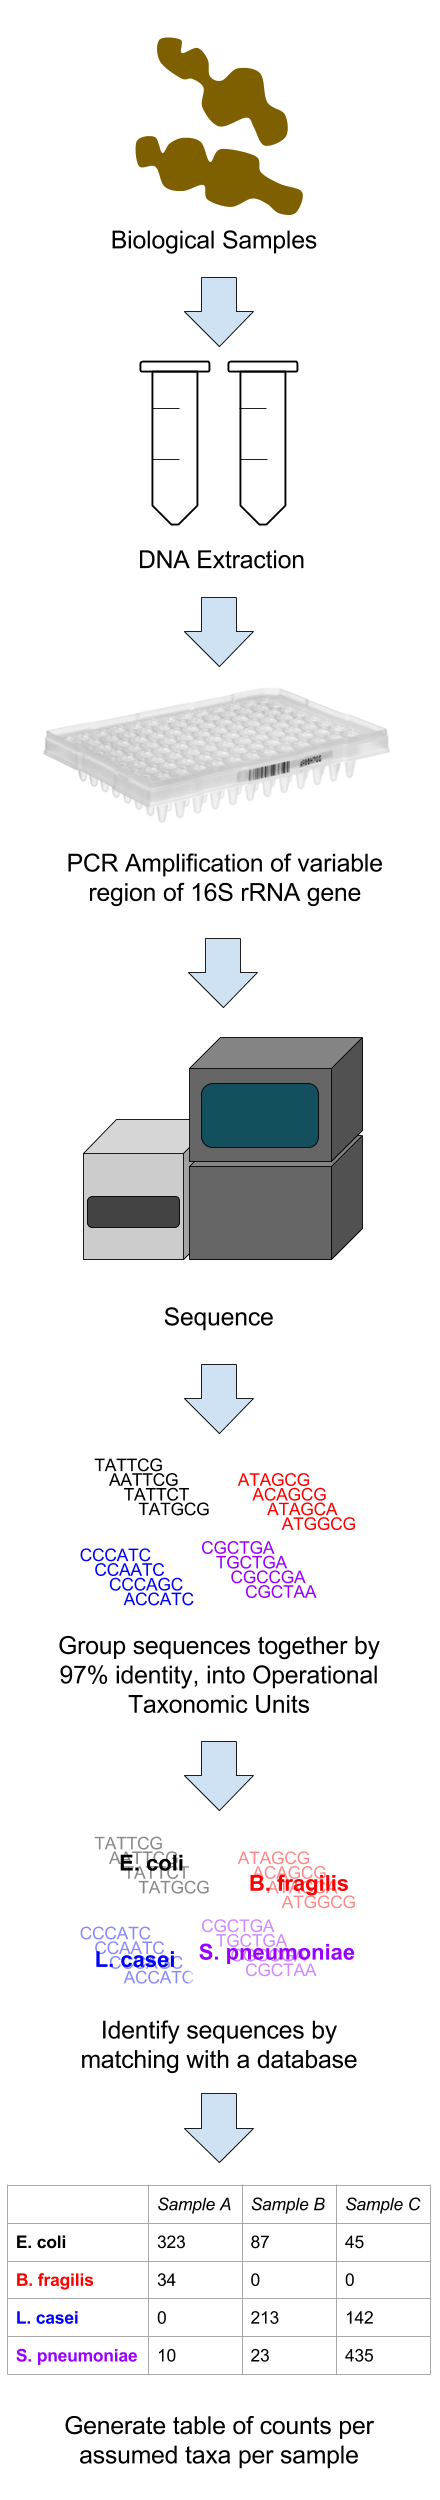
\includegraphics[width=0.95\textwidth]{16S_rRNA_pipeline.png}
\caption[16S rRNA gene tag experiment workflow.]{\textbf{16S rRNA gene tag experiment workflow.} This shows the workflow from sample collection to data generation. The end result is a count table of reads per operational taxonomic unit per sample.}
\label{16s_workflow}
\end{center}
\end{figure}

\begin{enumerate}
\item Take a biological sample and extract the DNA\\
The sample can be collected swabbing the target body site or by collecting samples in some other way. DNA extraction is usually done with common commercial kits.

\item Run a PCR amplification\\
As discussed previously, the gene tag experiments in this thesis amplify the V4 region of the 16S rRNA gene, following the Earth Microbiome Project protocol \cite{caporaso2012ultra}. The set of primers that we use are combinatorial barcoded, so that we can sequence all the samples in the same sequencing run and differentiate them afterwards \cite{gloor2010microbiome}.

\item Perform sequencing\\
We use 2x220 nucleotide paired-end sequencing on the Illumina MiSeq platform. The 220 nucleotide paired ends allow us to overlap paired sequences in the middle to reconstitute the full sequence of the V4 variable region, which is 298 base pairs in size.
\end{enumerate}

\paragraph{Post-sequencing processing}\mbox{}\\
Here are the steps for going from raw sequenced reads to a table of counts per taxa per sample.
\begin{enumerate}
\item Assemble the paired ends of sequenced DNA\\
The paired sequences are overlapped in the middle, resulting in the full variable region amplified by the primers.

\item Demultiplex the raw sequence\\
The barcodes are used to separate the sequences according to what sample they came from.

\item Group the reads into operational taxonomic units (OTUs)\\
We used UCLUST \cite{edgar2010search} to cluster the reads into groups of 97\% identity and UCHIME \cite{edgar2011uchime} to filter out chimeric sequences.

\item Annotate the OTUs with bacterial taxonomy\\
Annotation was done by  matching our OTUs to the SILVA database \cite{quast2013silva}.

\item Generate a phylogenetic tree\\
This can be done using the center-most sequence of each cluster that forms each OTU, and putting the sequences in a multiple sequence alignment, using software such as MUSCLE \cite{edgar2004muscle}. The multiple sequence alignment can be converted into a phylogenetic tree using software such as FastTree \cite{price2010fasttree}.
\end{enumerate}

Alternatively, an Individual Sequence Unit (ISU) based approach rateher than an OTU based approach can be taken, where the individual sequences are preserved even after grouping into OTUs, so that different strains within the same OTU can be analyzed separately \cite{callahan2015dada2}.

\FloatBarrier

\subsection{Data analysis}
There are two goals in gene tag data analysis. First, is there any structure in the data (separation, clustering, correlations, differentials, etc.)? Second, what drives the structure in the data?

Separation or clustering can be examined by determining the dissimilarity between each sample, and using these dissimilarities to plot the samples as points on a principal co-ordinate graph. The following sections will go over the most commonly used distance metric in microbiome research, called UniFrac, as well as the Principal Co-ordinate Analysis multidimensional scaling method for plotting the points on a graph. Afterwards the data can be visually or mathematically inspected for separation or clustering.

The technique used for determining if taxa are differentially abundant between groups is the same technique used for determining if gene annotations are differentially abundant between groups in the metagenomic experiment, and has its own section, titled \textit{Microbiome data is compositional}.

Principal Component Analysis (PCA) is a data reduction strategy used for multivariate statistics. However, the OTU abundances derived from the 16S rRNA gene sequencing experiment are proportional, so the PCA (which assumes a linear differences) is not applicable. Instead, the data must be transformed in some way into a Euclidean distance \cite{anderson2003canonical}. This is the rationale behind the development of the UniFrac distance metric. Using the pairwise UniFrac distances between the samples, a PCA can be performed to analyze the data.

\paragraph{UniFrac}\mbox{}\\
In 2005, Lozupone et al. introduced the UniFrac distance metric, a measure to calculate the difference between microbiomes that incorporated phylogenetic distance \cite{lozupone2005unifrac}. The goal of UniFrac was to enable objective comparison between microbiome samples from different conditions. In 2007, Lozupone added a proportional weighting to the original unweighted method \cite{lozupone2007quantitative}. Since then, papers reporting these metrics have garnered over a thousand citations, and enabled insights about everything from how kwashiorkor causes malnutrition \cite{smith2013gut} to how people can have a similar microbiome to their pet dog \cite{song2013cohabiting}.  Except for Generalized UniFrac, used to make hybrid unweighted and weighted UniFrac comparisons \cite{chen2012associating}, few advances in the metric have occurred since 2007. 

\paragraph{Unweighted UniFrac}\mbox{}\\

\begin{figure}[h]
\begin{center}
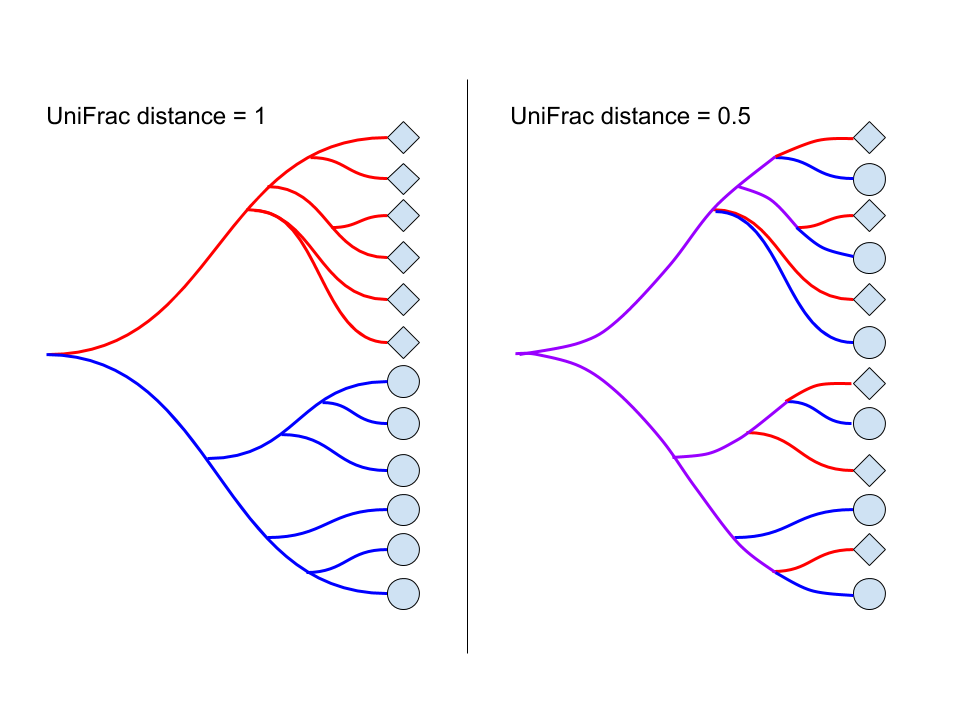
\includegraphics[width=\textwidth]{unifrac.png}
\caption[Unweighted UniFrac.]{\textbf{Unweighted UniFrac.} When two samples do not share any branches of the phylogenetic tree, the unweighted UniFrac distance is maximized at 1. When two samples share half of their branch lengths on the phylogenetic tree, the unweighted UniFrac distance is 0.5. If the two samples contain exactly the same taxa, the unweighted UniFrac distance is minimized at 0, since the samples share all branches.}
\label{unweighted_unifrac}
\end{center}
\end{figure}

Unweighted UniFrac uses an inferred evolutionary distance to measure similarity between samples (Fig. ~\ref{unweighted_unifrac}). It requires a reference phylogenetic tree containing all the taxa present in the samples to be examined. The calculation is performed by dividing the branch lengths shared between the two samples by the branch lengths covered by either sample. A distance of 0 means that the samples have an identical set of taxa detected, and a distance of 1 means that the two samples share no taxa in common.

The qualitative rather than quantitative nature of unweighted UniFrac makes the metric very sensitive to sequencing depth. A greater sequencing depth generally results in the detection of a greater number of taxa. To account for this problem, microbial ecologists use a technique called rarefaction to normalize the sequencing depth across samples by random sampling without replacement \cite{de2011evaluation}, although this is controversial \cite{mcmurdie2014waste}.

In the UniFrac paper, the authors pointed out that UniFac was unstable with rarefaction and recommended that users take the average of multiple UniFrac instances \cite{lozupone2011unifrac}. This is generally disregarded, sometimes even by the original authors \cite{mckenna2008macaque} \cite{mcnulty2011impact}.

\begin{figure}[h]
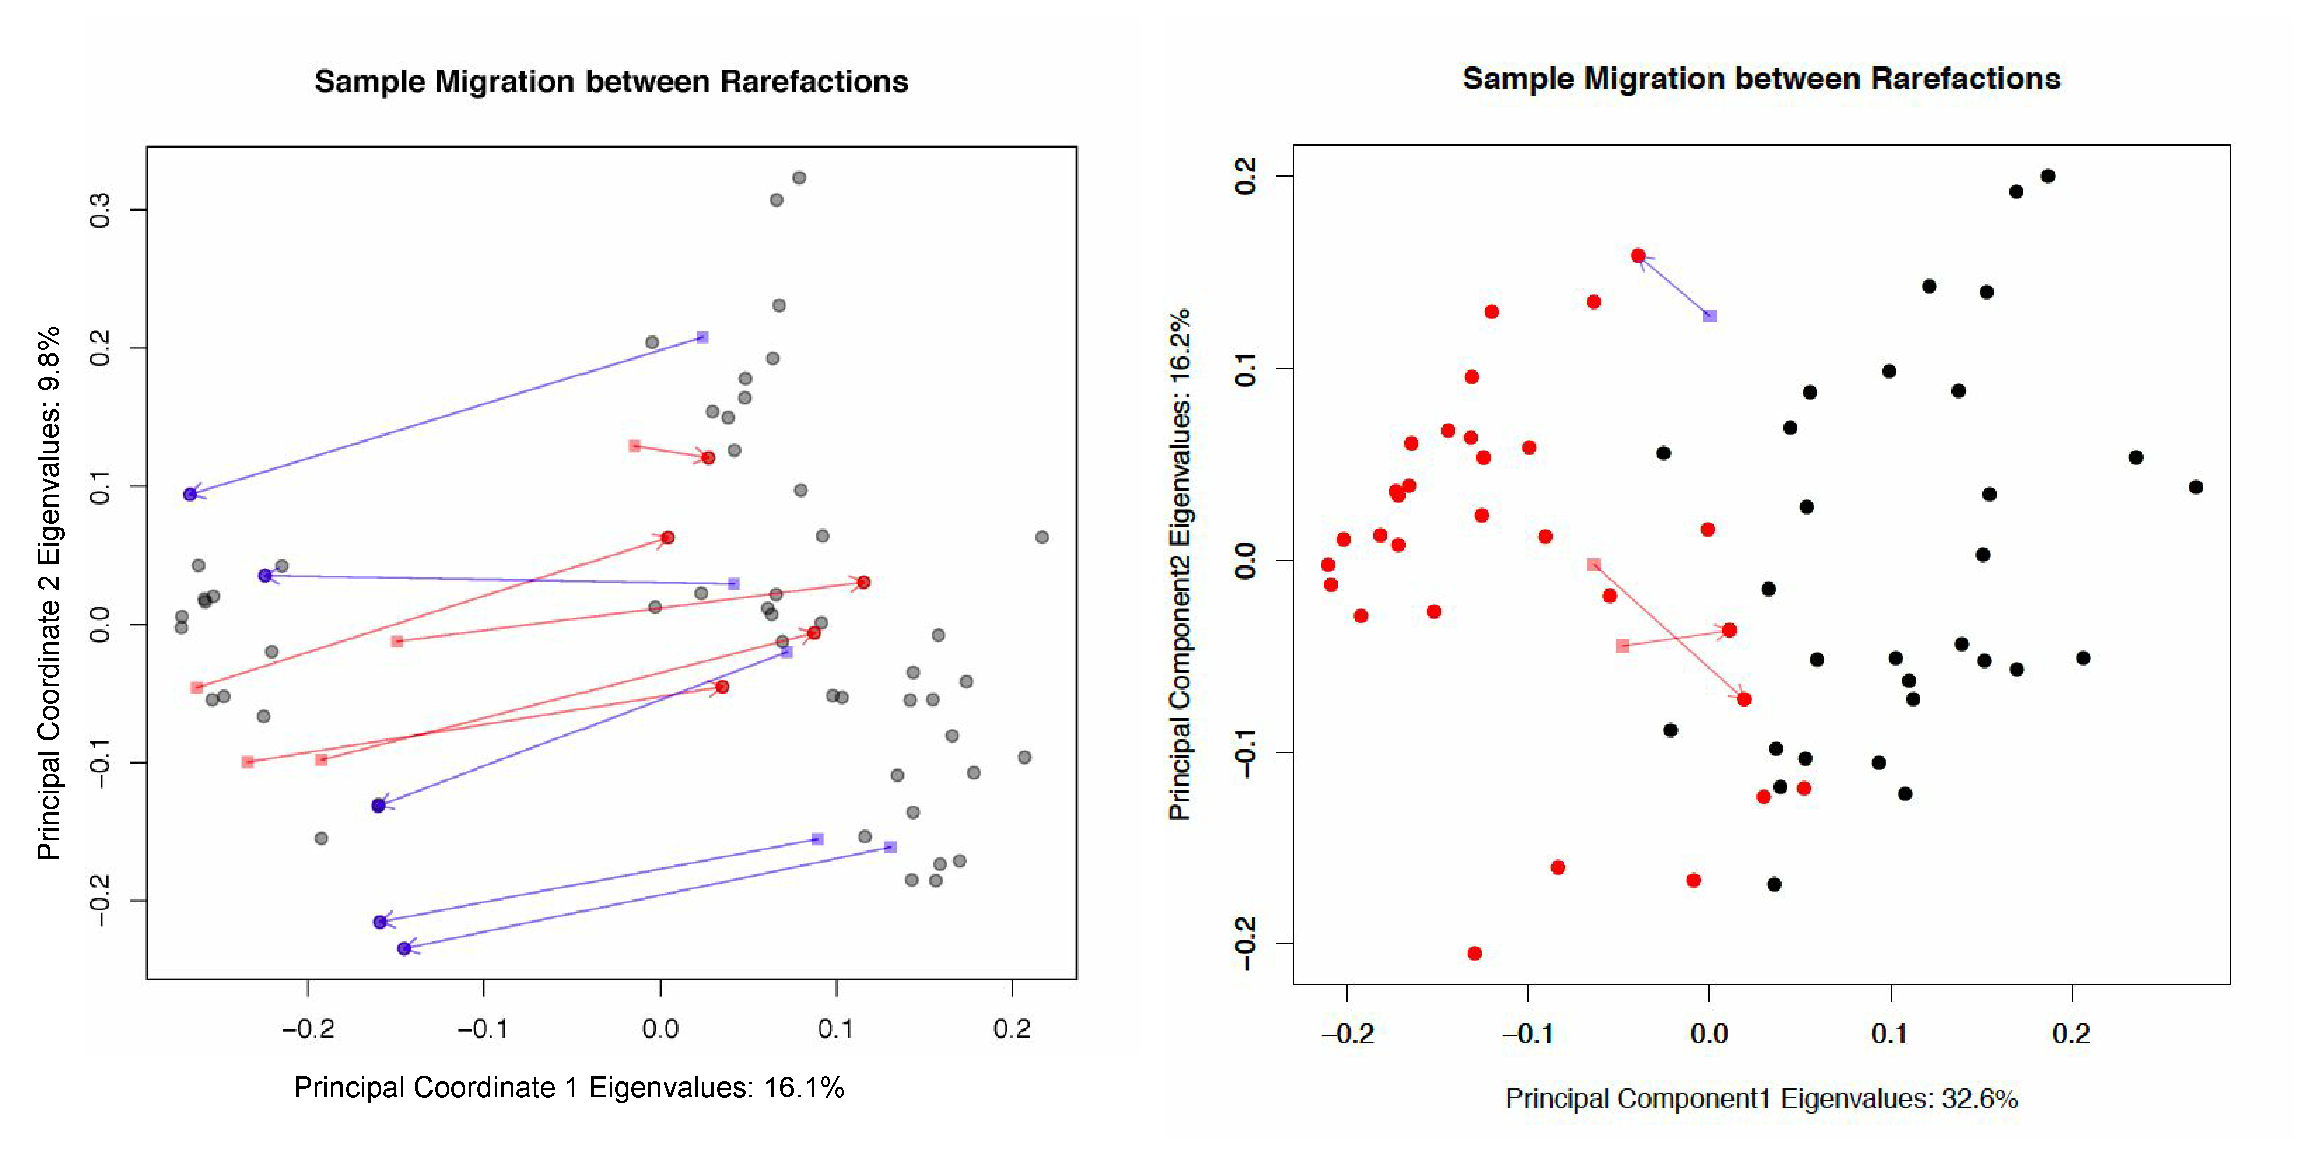
\includegraphics[scale=0.4]{sample_migration.eps}
\caption[Sample migration in different rarefactions, plotted on principal components, measured with unweighted UniFrac.]{{\bf Sample migration in different rarefactions, plotted on principal components, measured with unweighted UniFrac.}
The left panel shows the movement across clusters for a set of randomly selected tongue dorsum samples from healthy volunteers in the Human Microbiome Project database. The right plot has samples from tongue dorsum and buccal mucosa, which have real separation. If the tongue only experiment were run once, one might mistakenly assume that there are two clusters of data, however, the inconsistent sample membership of the two groups between rarefactions proves the clustering irreproducible. Note that the variance explained in the tongue data set by the first and second component is merely 16.1\% and 9.8\% respectively, indicating that the data is rather spherical, even though the points on the plot appear to show two separated clusters.}
\label{figure_sample_migration}
\end{figure}

In unweighted UniFrac, samples move relative to the other samples in different rarefaction instances, to the point where they can switch from being a member of one cluster of data to another (Fig. ~\ref{figure_sample_migration}). Any published finding done with an unweighted UniFrac analysis is suspect, especially if only one rarefaction instance is reported or if most of the variance is not explained by the first and second principal components. This is further explored in the chapter \textit{Expanding the UniFrac Toolbox}.

\FloatBarrier

\paragraph{Weighted UniFrac}\mbox{}\\

\begin{figure}[h]
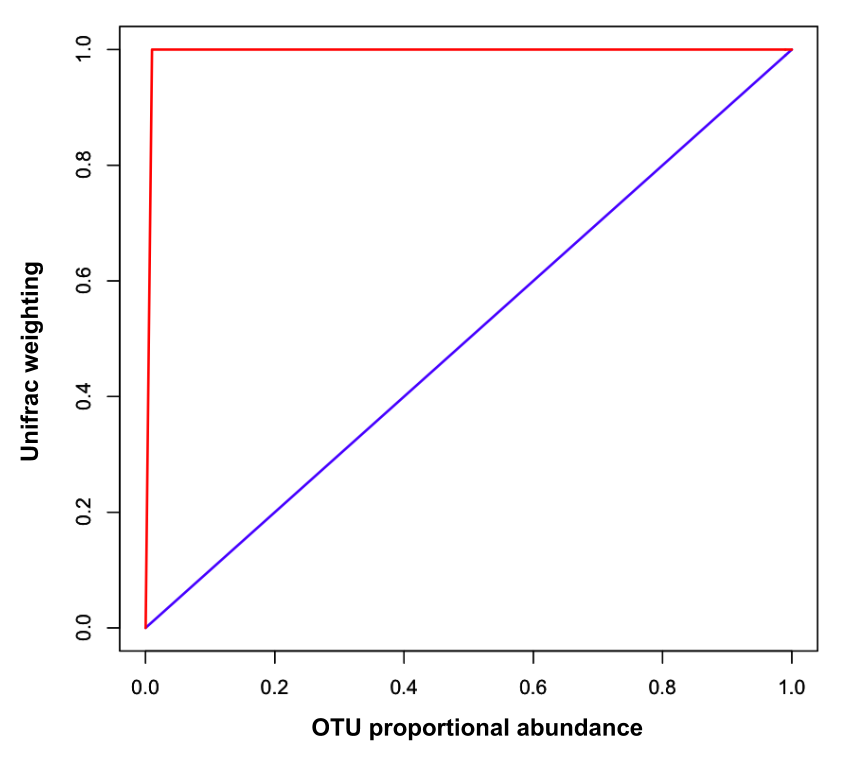
\includegraphics[scale=0.5]{weights.png}
\caption[Unweighted vs. weighted UniFrac weights.]{{\bf Unweighted vs. weighted UniFrac weights.}
The solid line represents the weight that unweighted UniFrac would produce with the given proportional abundance, and the dotted line represents the weight that weighted UniFrac would produce.}
\label{figure_weights}
\end{figure}

Weighted UniFrac is an implementation of the Kantorovich-Rubinstein distance in mathematics, also known as the earth mover's distance \cite{evans2012phylogenetic}. Rather than looking only at the presence or absence of taxa, each branch length of the phylogenetic tree is weighted by the difference in proportional abundance of the taxa between the two samples (Fig. ~\ref{figure_weights}). This technique reduces the problem of low abundance taxa being represented as a 0 or by a low count depending on sampling depth. In unweighted UniFrac, such taxa would flip from absent to present, and could skew the measurement: this would be especially problematic if the taxa are on a long branch. In weighted UniFrac, low abundance taxa have a much lower weight and so will have a reduced impact on the total distance reported by the metric.

UniFrac is constituted as either a presence/absence (unweighted UniFrac) \cite{lozupone2005unifrac}, a linear proportion in the form of weighted UniFrac \cite{lozupone2007quantitative}, or some combination of the two in the form of Generalized UniFrac \cite{chen2012associating}. However, the data are not linear, because the sum of the total number of reads is constrained by the sequencing machinery \cite{friedman2012inferring}. Alternative weightings and nonlinear transformations of data need to be explored, and this is the focus of Chapter 2.

\paragraph{Principal Co-ordinate Analysis}\mbox{}\\
Once the dissimilarity between each pair of samples has been calculated, they can be visualized on a plot, with each sample represented as one point. For visualization, the data should be placed so distances are preserved as much as possible, so that clustering and separation of samples can be clearly seen. This is done using the Principal Co-ordinate Analysis method of multidimensional scaling \cite{dollhopf2001interpreting}, shortened as PCoA. PCoA is a singular value decomposition of the distance relationships.

To plot all of the samples as points in space such that the distances between each pair of samples are preserved, multiple dimensions are required. In this data specifically, the number of dimensions required is equal to one less than the number of samples. PCoA rescales all the dimensions as components, so that the first component captures the largest distances, or spread of the data, the second component captures the largest distances remaining in the data after the first component, and so on. This way, even if only the first two components are used to plot all the samples as points on a two dimensional graph, the data is spread out to enable visualization of separation or clustering. Ideally the first and the second principal components should explain most of the distance in the data. For example, there is much less variance explained in the uniform tongue dorsum data set, compared to the data set with separation between tongue dorsum and buccal mucosa samples (Fig. ~\ref{figure_sample_migration}).

After multidimensional scaling the data can be analyzed in several ways. The data can be examined by k-means analysis clustering \cite{tibshirani2005cluster} or by unsupervised clustering.

The points can also be measured for separation by looking only at their position on the first principal component axis, especially if the first axis covers the majority of the variation in the data set. With each sample associated with a number on the first principal component axis, one can examine the effect size of two different groups by taking the mean positions and dividing by the standard deviation.

There are several limitations of principal co-ordinate analysis. First, it is an indirect analysis. If a separation between groups is found, further examination is necessary to determine the source of separation. Second, the PCoA is only as good as the dissimilarity metric used. Lastly, one cannot easily determine the contributions of each OTU to the principal components.

\section{The metagenomic experiment}
Deep metagenomic sequencing provides an estimate of the proportion that each type of gene composes out of the total genes present in the genetic material of the sample. This can be used to answer questions such as:

\textit{What is the metabolic potential of the microbial community?}
The metabolic potential is made up of all the protein functions that are encoded by the genetic material present in the sample. Biologically speaking, these protein functions represent the enzymatic reactions that the microbiome could produce if all the genes were expressed. For example, the human gut microbiome is known to facilitate methanogenesis. However, methanogenesis is a common function in rare taxonomic groups (mostly \textit{Archaea}). Metagenomic sequencing shows that the human gut microbiome has more genes related to methanogenesis than expected - a feature that would have not been as prominent in 16S rRNA gene sequencing analysis \cite{gill2006metagenomic}.

\textit{Are any genes, functional categories of genes, or metabolic pathways made up of genes differentially abundant between groups?}
In 2006, Turnbaugh et al. published a paper showing that an obesity associated gut microbiome in mice had an increased capacity for energy harvest \cite{turnbaugh2006obesity}, sparking more research into the gut microbiome and obesity related ailments such as diabetes \cite{larsen2010gut} and nonalcoholic fatty liver disease \cite{zhu2013characterization}. The ability to check if genes, functional categories of genes, or pathways are differentially abundant between groups allows scientists to find clues about the mechanisms by which the microbiome affects certain diseases.

All of this information can be determined by either imputation or actual sequencing, discussed in the next sections.

\subsection{Sequencing}

\begin{figure}[h]
\begin{center}
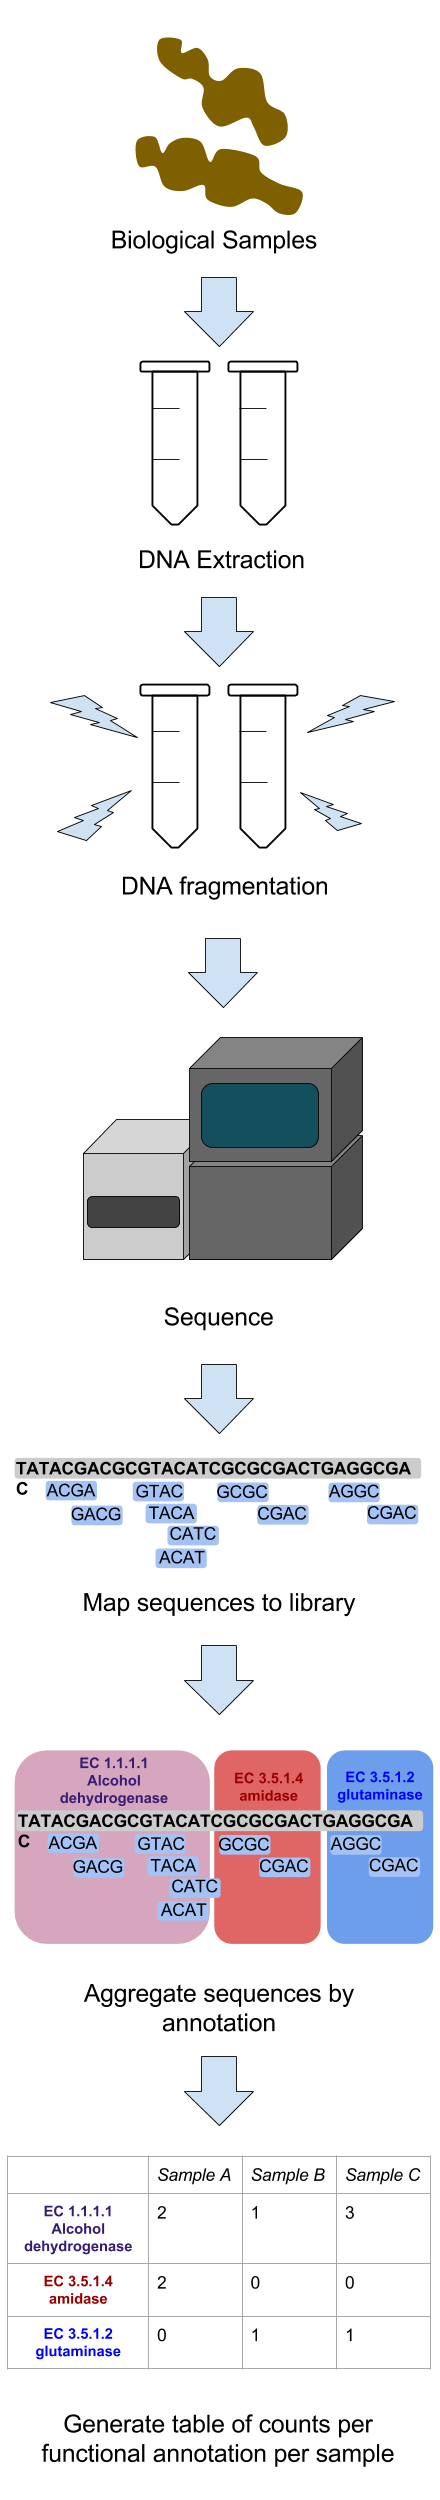
\includegraphics[width=0.95\textwidth]{Metagenomic_pipeline.png}
\caption[Metagenomic experiment workflow.]{\textbf{Metagenomic experiment workflow.} This shows the workflow from sample collection to data generation. The end result is a table of number of sequencing reads per functionally annotated gene per sample.}
\label{metagenomic_workflow}
\end{center}
\end{figure}

The goal of metagenomic DNA sequencing analysis is to examine the metabolic potential of the microbiota in the microbiome. This is done by identifying genes by DNA sequence, sorting them by the known function of the protein that they encode (such as the catalysis of a certain reaction), and checking if any functions are differentially abundant between conditions. Further analysis can also include checking for pathway enrichment, and assembling the sequenced reads into genomes. The general protocol for metagenomic analysis (Fig. ~\ref{metagenomic_workflow}) is as follows:

\begin{enumerate}
\item Take a biological sample and perform DNA extraction\\
The sample can be collected by swabbing the target body site or collecting excretions.

\item Prepare the DNA for sequencing\\
Fragment the DNA, and filter for the desired size. These steps are all part of the standard Illumina library prep protocol for the HiSeq.

\item Sequence the DNA.\\
We performed single end sequencing on the Illumina HiSeq platform, with our samples barcoded so that they could be pooled into the same sequencing run. There are two options for read length: either 50 or 100 nucleotides. We chose the longer one for ease of assembly and mapping.

\item Create an annotated library of reference sequences\\
The annotated library contains DNA sequence annotations about what kind of protein each sequence codes for. The first step to creating the annotated library is to gather a database of sequences. The database of sequences can be created before the sequencing is complete by gathering all the genomes of all the bacterial strains predicted to be present in the sample, or it can be created after sequencing by assembling the sequenced reads into parts of genomes. The second step is to annotate the sequences with predicted protein functions. Most publically available genomes already have protein annotations. For genomes or partial genomes without annotations, the placement of genes can be predicted by looking for open reading frames, and these predicted genes can be aligned with databases such as SEED \cite{overbeek2005subsystems} or KEGG \cite{kanehisa2000kegg} to match them with functional annotations, using the BLAST algorithm \cite{altschul1990basic}.

\item Map the sequenced reads to the library\\
Mapping is the process of annotating the sequenced reads by aligning them with sequence that has already been annotated. We used Bowtie2 \cite{langmead2012fast} to map our sequenced reads to the annotated library created in the previous step. Bowtie2 aligns similar sequences together.

\item Determine how many mapped reads match each functional annotation\\
Once the sequenced reads have been mapped to the annotated reference sequence, the number of reads sequenced for each annotation can be counted up. The end result is a table of counts per gene annotation per sample.
\end{enumerate}

Issues with sequencing and the analysis of sequencing data arise from sampling and the ``fat'' nature of the data.

The DNA has been randomly sampled multiple times before the sequencing data is retrieved: The biological sample collected from the patient is only part of the full bacterial community. The amount of DNA extracted is a sample of that sample. Only a fraction of the extracted DNA is sequenced, and finally the DNA fragments that the sequence reads are sampled out of the input DNA. As a result, on top of the biological variation present in the microbiomes being sampled, there is an additional layer of technical and random variation. High variation or noise in the data can obscure small but biologically significant differences between experimental conditions.

Additionally, primers used for sequencing may be biased for certain sequences more than others \cite{kanagawa2003bias}. Lastly, the data is very fat, which is to say that there are many more variables (in the form of functional annotations of genes) than there are samples. This makes it difficult to have enough power to detect small differences in the data, a concept expanded upon in the \textit{Microbiome data involves the comparison of many features} section.

\FloatBarrier

\subsection{Imputation}
When it is not financially feasible to perform deep metagenomic sequencing, the sequencing results can be imputed using a tool called PICRUSt from a gene tag experiment \cite{langille2013predictive}. PICRUSt uses the Greengenes database \cite{desantis2006greengenes} to identify the bacterial taxa in the sample, and pulls their genomes from the Integrated Microbial Genomes database \cite{markowitz2012img}. With the genomes, the program tries to predict what would be seen if the samples underwent deep metagenomic sequencing. For taxa without a fully sequenced genome, PICRUSt infers the genetic content based on ancestors in the phylogenetic tree. PICRUSt produces metagenome predictions with a Spearman correlation coefficient of about $0.7$ \cite{langille2013predictive}, compared to a full metagenomic sequencing experiment.

Imputation is useful for identifying potential correlations that should be explored and validated further, but should not be used to make conclusions. The issues with imputation include all the issues with sequencing, plus the added variation in its imperfect correlation.

\subsection{Data aggregation, categorization, and amalgamation}
Data analysis can be performed to determine if functions are differentially abundant between samples in different groups (described in the \textit{Microbiome is compositional} section), examining functional categorizations, and checking for pathway enrichment. Sequenced genes (open reading frames) can be grouped by common function through annotation by querying the SEED or KEGG functional annotation databases. These functions can be analyzed to see if any are differentially abundant between experimental conditions.

\paragraph{Functional categorization}\mbox{}\\

\begin{figure}[h]
\begin{center}
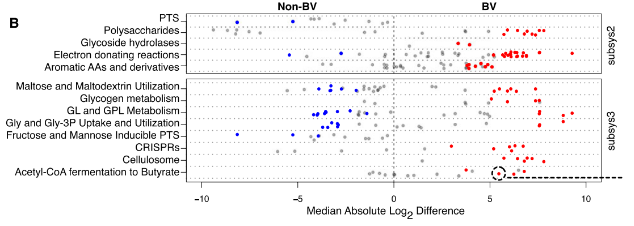
\includegraphics[width=\textwidth]{stripchart.png}
\caption[Example stripcharts for subsystem 2 and 3 functional categorizations.]{\textbf{Example stripcharts for subsystem 2 and 3 functional categorizations.} Dots on the left side are SEED subsystem 4 annotations found to be more abundant in the healthy condition while dots on the right side are subsystem 4 annotations found to be more abundant in the bacterial vaginosis condition. Colored dots were found to be significantly differentially abundant. Figure taken from \cite{macklaim2013comparative}.}
\label{stripchart_example}
\end{center}
\end{figure}

We typically use the SEED annotation, which has four different levels of categorization. Subsystem 4 is the most atomic categorization level and describes the specific function of the protein group, for example, “Isovaleryl-CoA dehydrogenase (EC 1.3.99.10)”. Subsystem 3, 2, and 1 are increasing more general levels of categorizations, from enzyme families to large categorizations such as genes related to carbohydrate metabolism. These levels are simply aggregations of subsystem 4 levels, and one subsystem 4 annotation can be found in one or more higher level groups.

An effect size is measured by taking the difference in means between two groups of data, and dividing by the standard deviation within groups. The effect size is stronger when there is less overlap between the two groups. Even if the subsystem 4 functional categories are not significantly different between groups, they each have an effect size with a direction. Stripcharts can be used to plot the effect sizes of the subsystem 4 categories for a larger category (Fig. ~\ref{stripchart_example}). For example, by plotting the effect sizes of all the subsystem 4 categorizations under Carbohydrate Metabolism, one can visually see if there are any obvious directional trends for carbohydrate metabolism functions being relatively abundant in the experimental group compared to the control.

\FloatBarrier

\paragraph{Pathway enrichment}\mbox{}\\
Biological pathways can be thought of as made up of a series of chemical reactions, each catalyzed by a protein enzyme, which is encoded by a gene. KEGG (Kyoto Encyclopaedia of Genes and Genomes) is a manually curated annotation database that matches genes to pathways \cite{kanehisa2000kegg}. This database allows researchers to see if there is differential abundance of pathways encoded by functionally annotated genes, even when the genes may not be differentially abundant by themselves. This is an alternate amalgamation of the data.

\section{Points of failure}
The Huttenhower lab has organized the Microbiome Quality Control project (MBQC) at http://www.mbqc.org/. Preliminary results show that despite being given the same samples, different participating labs can come up with vastly different results. This lack of reproducibility is caused by a lack of consensus on the correct way to analyze microbiome data. The following sections explore different aspects of microbiome collection, sequencing, and data that contribute to this.

\subsection{Collection methods differ}
The 16S rRNA gene sequencing experiments are very sensitive to batch effects. Microbiome composition is often naturally highly diverse between different individuals. The high amount of variation means that the effect size of a difference between groups can be small \cite{fernandes2014unifying}. Next generation sequencing is also a sensitive technology, and the data can be confounded by contaminants \cite{salter2014reagent} or batch effects. These artifacts can overpower real biological effects. Wherever possible, all samples should be processed in the same batch. Analysis should also be done to check if samples extracted on different dates or sequenced with different primers separate into clusters, to make sure that there is no systematic bias in the data.

\subsection{Microbiome data is highly variable between individuals}
The gut is often studied but the gut microbiome can be affected very strongly by diet \cite{turnbaugh2009effect}. This among other factors lead to a highly diverse gut microbiome between subjects for reasons unrelated to the disease being studied. This can create a lot of variability, potentially obscuring real effects or even creating the appearance of false effects.

Generally experiments of this nature typically have low sample sizes due to budget constraints, sample collection difficulties, patient compliance, and other issues. To increase cost effectiveness and reduce batch effects (such as from kit contamination \cite{salter2014reagent}), we run all the samples in an experiment on the same sequencing run, by means of a combinatorial barcode primer design \cite{gloor2010microbiome}.

There are several models for computationally analyzing the variance within conditions in order to determine if operational taxonomic units are significantly differentially abundant, such as LEfSe \cite{segata2011metagenomic} and Metastats \cite{paulson2011metastats} for microbiome analysis. Most of these were originally designed for RNA-seq experiments on single organisms \cite{pachter2011models}. Currently the most popular tools for analyzing differential abundance are EdgeR \cite{robinson2010edger}, DESeq2 \cite{love2014moderated}, MetagenomeSeq \cite{paulson2014metagenomeseq}, and LEfSe \cite{segata2011metagenomic}. EdgeR was cited by 52 papers that mentioned the microbiome in 2015 according to Google Scholar. DESeq2 and MetagenomeSeq are part of the QIIME pipeline, which was cited by 1,080 microbiome papers in 2015. LEfSe has been cited by 145 microbiome papers in 2015.

EdgeR and DESeq2 use the negative binomial distribution. The negative binomial distribution allows the variance of data to be estimated given the mean, through a function. The function is determined by collecting the mean and variance for all the counts for each OTU in each experimental condition, and fitting the variances according to the negative binomial distribution. This vastly underestimates the variance at low counts, which represent the sampling of low abundance OTUs, and can be very different between replicates. Underestimating the variance at low counts produces spurious low p-values for low count OTUs \cite{fernandes2013anova}.

MetagenomeSeq uses the Zero-Inflated Gaussian (ZIG) model, which is a binomial distribution of counts (that may include zero counts), plus a function to predict how many extra zeros there will be. This does not work well when the total number of reads are not well matched, because then there will be many more zeros in the data set with less reads, due to having a lower sequencing depth, and a consistent total read count is required between samples according to page 2 of the supplementary material in the first metagenomeSeq paper \cite{paulson2014metagenomeseq}.

LefSe stands for the Linear discriminant analysis (LDA) Effect Size method \cite{segata2011metagenomic}. It identifies significantly differentially abundant OTUs, checks for consistency in the differential abundance with the Wilcoxin rank sum test, and uses linear discriminant analysis to estimate an effect size per feature. This method assumes that microbial communities can be split by a linear combination of OTUs (for example the line $ax + by$, where $a$ and $b$ are constants and $x$ and $y$ are OTU abundances). However, bacterial abundances in both count form and proportions do not grow at a linear rate.

EdgeR, DESeq2, and MetagenomeSeq all work by using a statistical model to make a point estimate of the mean and variance of the data. Using the estimated mean and variance, differential abundance is tested statistical significance. However, a point estimate obscures technical variation in the data. That is, if a technical replicate were performed by resequencing the samples, a different set of point estimates would be calculated. In contrast, Bayesian methods model the distribution of the mean and variance.

For my differential abundance analysis, I’ve used ALDEx2, which samples from the Dirichlet distribution to model variation in the data \cite{fernandes2014unifying}. After a number of samples, the mean value and mean variance are used to determine if OTUs are differentially abundant between groups, an approach that is believed to result in greater specificity and equivalent sensitivity compared to the point estimate approach \cite{fernandes2014unifying}.

\subsection{Microbiome data involves the comparison of many features}
Oftentimes, the number of taxa or gene functions is more than a magnitude larger than the samples. This is known in statistics as having more variables than observations, or having fat data. The higher the ratio of variables to observations are, the less likely the principal components analysis or pairwise comparison is to be reliable \cite{osborne2004sample}.

One way to conceptualize the problem is through combinatorics. Hypothetically, there could exist many bacterial taxa that are equally present in both conditions, but have a low abundance such that a 0 or 1 count is often detected. In this case the chances of observing all 0 counts in one condition and all 1 counts in another condition by simple combinatorics is quite high. This situation is common in microbiome data, where most of the bacteria are abundant in low proportions, sample sizes are often low, and a typical 16S rRNA gene sequencing experiment detects hundreds of OTUs.

Multiple test corrections assume that the experiment has more samples than variables, and result in very high p-values when this condition is not met. However, when using p-value based tests, researchers should include multiple test corrections to ensure that the results they are reporting are not all false positives. Unfortunately many studies have been published in peer reviewed journals without multiple test corrections. For example, four out of five papers in the literature about the gut microbiome and non-alcoholic fatty liver disease did not use a multiple test correction (Fig. ~\ref{introduction_nafld_fig1}).

\subsection{Microbiome data is compositional}
In both gene tag sequencing and metagenomic sequencing experiments, the data is in the form of a list of counts per feature, with the features composing an aspect of the microbiome for each sample. Therefore, the number of counts observed is arbitrary and not related to number of counts in the original environment. For example, an oral sample ($10^{7}$ Colony Forming Units/ml) and a gut sample ($10^{10}$ CFU/ml) will give same number of counts (~$1 \times 10^{5}$) after DNA sequencing. This is compositional data. There are several core truths about microbiome data and its compositional nature that should be considered when making an analysis strategy.

First, the total number of reads per sample is irrelevant to the biological implications of the data. The number of reads is determined mainly by the chosen sequencing platform (i.e. Roche 454, Illumina MiSeq, or Illumina HiSeq). The absolute abundance of reads per sample cannot be used to make biological inferences.

Second, spurious correlations can arise from proportional microbiome data, and should be avoided. In the late 19th century, many studies were being published about how organ sizes (normalized by dividing the size by the individual's height) were correlated. However, it was discovered that when two sets of uncorrelated data are both divided by a third set of uncorrelated data, the two sets will appear spuriously correlated \cite{pearson1896mathematical}. This is analogous to microbiome data where raw counts are normalized by dividing by the total number of counts \cite{pearson1896mathematical}.

\begin{figure}[h]
\begin{center}
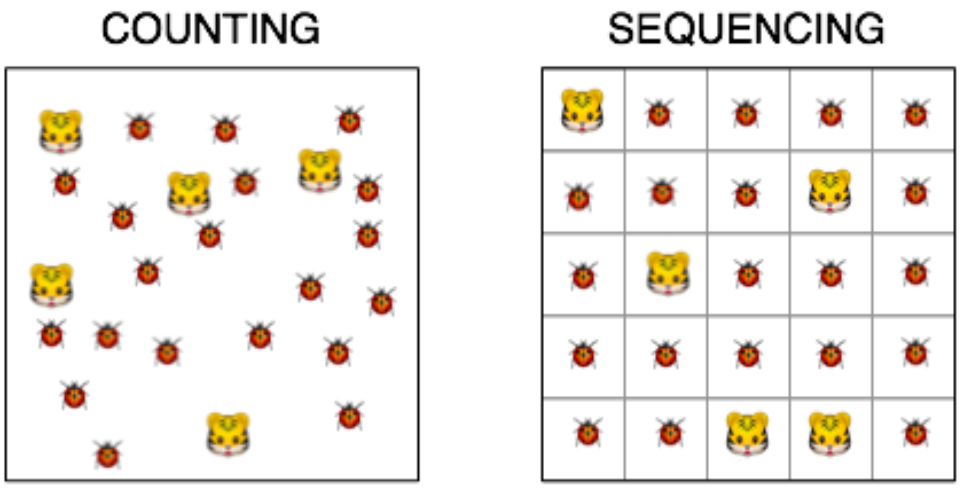
\includegraphics[width=0.7\textwidth]{lions_ladybugs.png}
\caption[Counting vs. sequencing.]{\textbf{Counting vs. sequencing.} In ecology, where all the animals in a given area are counted, there is no upper limit on the number of animals that can be detected. In sequencing, there is a constraint on the total number of sequences detected by the sequencing platform. If one were to detect one more ladybug, one would have to detect one less lion. Figure courtesy of Dr. Greg Gloor, \url{http://gloorlab.blogspot.ca/2016/04/sequencing-is-not-counting-idea-of.html}.}
\label{introduction_lions_ladybugs}
\end{center}
\end{figure}

Additionally, the constrained sum causes the abundance of different taxa to appear to be negatively correlated with each other when analyzed by conventional statistics. When one taxa increases in abundance, the counts detected in other taxa decrease in proportional abundance, even if the taxa are not decreasing in absolute abundance biologically. This negative correlation bias arises when the data are treated as univariate, when it should be analyzed as multivariate data. All non-parametric tests (Principal Co-ordinates Analysis, correlations, etc.) assume that the abundance measured for each feature is independent. This is true in ecology where the abundance of different species is measured in an area of land where animals can move freely in and out. It is not true in next generation sequencing where the abundance of different species is measured by a sequencing platform with a limited number of measurements, such that detecting extra members of one species means detecting less members of another species (Fig. ~\ref{introduction_lions_ladybugs}).

Third, removing an entire variable (an OTU in gene tag sequencing, or a functional annotation in deep metagenomic sequencing) from the analysis should not change correlations between OTUs. This is true with counts but not true with proportions \cite{lovell2015proportionality}. A correlation between two OTUs is suspect if it is dependent on the presence of an additional unrelated OTU. Removing variables occur routinely in microbiome research. For example, rare OTUs are thought to not be very informative, and low counts have high variability, so they are often filtered out. Additionally, primers may be biased against certain taxa, which are underrepresented in the data. Finally, some experiments are performed only on taxa of interest (as is the case with qPCR), and all other OTUs are not considered in the analysis. Without the proper data transformation, removing variables from the full set will change the correlation between variables \cite{aitchison1982statistical}.

To ensure that these conditions are met, data should be analyzed in a compositional way. In Euclidean space, data points can increase or decrease freely. Compositional data is under a sum constraint, and exist in a non-Euclidean space known as the Aitchison simplex \cite{aitchison1982statistical}. Many operations are not valid for data on a simplex. These include addition and subtraction, covariance, and correlation. A data transformation can be performed to put the data into Euclidean space, so that it can be analyzed with standard statistical methods that depend on Cartesian co-ordinates and linear relationships.

Several types of log ratio data transformations are recommended to allow the data to be analyzed by standard Euclidean methods \cite{aitchison1982statistical}. The type that makes the most sense for microbiome data is the centered log ratio transform. The centered log ratio transform is performed by dividing each proportional abundance by the geometric mean of all the proportional abundances, and taking the logarithm. Here $x_i$ is one proportional abundance within a sample, and there are $n$ OTUs in total.

\begin{align*}
clr(x_i) = \frac{x_i}{\sqrt[n]{\prod_{i=1}^{n} x_i}}
\end{align*}

The geometric mean acts as a baseline abundance in microbiome data. Taking the logarithm of the ratio allows for a symmetric measurement whether the large number is in the numerator or denominator of the ratio.

The centered log ratio transform prevents the total number of reads from affecting the measurement, so long as the geometric mean is a relatively stable baseline. The geometric mean is stable when the total number of reads is constant, or the per feature variation is random. The latter condition is met in a typical microbiome data set. The centered log ratio transform also allows for coherent subcompositional data analysis as the ratios between the remaining values are not affected when entire variables are removed. Note that a logarithm cannot be performed when the data contain one or more zero counts, which is problematic as microbiome data is sparse. This issue is discussed in the next section.

Compositional techniques such as those espoused in the ANOVA-Like Differential Expression 2 (ALDEx2) software \cite{fernandes2014unifying} and the Analysis of Composition of Microbiomes (ANCOM) framework \cite{mandal2015analysis} should be used to promote consistent data analysis. ALDEx2 models the technical variation using the Dirichlet distribution and then performs a log ratio transform while ANCOM uses log ratio analysis to make point estimates of the variance and mean, without any distributional assumptions.

However, these techniques are not yet mainstream in the field, resulting in many conclusions that are not reproducible. One example of this is referenced in the chapter about the gut microbiome and non alcoholic fatty liver disease, where five papers have been published on the same topic with almost completely non overlapping results (Fig. ~\ref{introduction_nafld_fig1}).

\subsection{Microbiome data is sparse}
One of the fundamental challenges in analyzing differential abundance is accounting for zeroes. Unlike a presence/absence test, a zero does not necessarily mean that the OTU is not there. The OTU could be present in an amount smaller than the resolution of the test, or it could be present but missed due to random sampling. This is a problem because when statistical methods are used to examine significantly different OTU abundance, as the comparison of zero values to non-zero values are likely to come out as significant whether or not the OTU abundance is differential. However, a 0 and a 1 count are easily interchangeable between technical replicates and the difference is not biologically significant \cite{gloor2016s} \cite{fernandes2013anova} \cite{fernandes2014unifying}. Additionally, the log transformations used in compositional data analysis cannot be performed on zeros. Statisticians often recommend that any sample with at least one zero count be removed during compositional data analysis, but for microbiome data this would often result in the removal of all the samples \cite{aitchison1982statistical}.

One solution to make zeros compatible with a compositional data log transformation is to add a small arbitrary value to each zero \cite{aitchison1982statistical}. The value used can be 0.5, representing uncertainty as to whether the zero represents an absence of the feature or if the feature is actually present but was missed due to random sampling or sequencing depth. In a Bayesian model, the 0.5 value is a prior. The second method is to estimate the likelihood that a zero was observed because of sampling depth. This is implemented by the cmultRepl command in the zCompositions package in R, with the `count multiplicative zeros' option \cite{palarea2015zcompositions}.

The microbiome field is quite new, and has been undergoing many exciting developments. Gold standards must be set to ensure that studies are replicable, and that published research represents the biological reality.

\section{The gut microbiome in patients with nonalcoholic steatohepatitis compared to healthy controls}
Non alcoholic fatty liver disease (NAFLD) has been on the rise along with obesity, affecting a fifth to a third of the North American population \cite{preiss2008non}. Most people with NAFLD remain asymptomatic, however, in up to a third of patients NAFLD can progress to nonalcoholic steatohepatitis (NASH), causing inflammation and scarring (fibrosis) in the liver, and decreasing the 5 year survival rate to 67\% \cite{propst1995prognosis}. It is thus important to shed some light on the process by which people progress from NAFLD to NASH to find interventions that prevent NASH.

There are several known genetic and chemical factors that increase the risk of progression to NASH in animal models and humans.

In mice non alcoholic fatty liver disease is often modelled with a methionine/choline-deficient diet (MCD), which induces steatohepatitis in wild type mice. Mice with a toll-like receptor 4 knockout had lower lipid and injury accumulation markers when fed a MCD diet \cite{rivera2007toll}. In rats liver fibrosis can be induced by drugs. One study found that male rats were more prone to this induced liver fibrosis than female rats. Fibrosis biomarkers were reduced when the male rats were dosed with estradiol, and increased when the male rats were additionally given an estradiol-neutralizing antibody. Female rats who had their ovaries removed similarly lost the protective effect \cite{yasuda1999suppressive}. From this, hormones are also a factor in nonalcoholic fatty liver disease progression.

In humans, the I148M variant of the Patatin-Like Phospholipase Domain Containing 3 gene (PNPLA3) correlates with a 3.2 fold increased risk of progression to NASH from NAFLD when homozygous, compared to to patients without the variant \cite{sookoian2011meta}. The heterozygous gene was found to be associated with fatty liver disease in genome wide association studies, but some additional studies have failed to replicate the relationship with NASH \cite{sookoian2011meta}. On the epigenetic level, many genes are differentially methylated in the livers of patients with advanced NAFLD compared to mild NAFLD. Eleven percent of genes are differentially hypomethylated in advanced NAFLD (compared to 3\% hypermethylated), leading to increased expression \cite{murphy2013relationship}. In advanced NASH specifically, some tissue repair genes were hypomethylated while some metabolism pathways such as 1-carbon metabolism were hypermethylated. However, only 7\% of the differentially methylated genes were found to be differentially transcribed \cite{murphy2013relationship}.

On a metabolite level, Raman et al. found differences in the number of volatile organic compounds detected in patients with NAFLD compared to obese patients without NAFLD \cite{raman2013fecal}. Reactive oxygen species have also been implicated in NASH due to their involvement in the mechanism of steatohepatitis-inducing drugs \cite{berson1998steatohepatitis}.

The microbiome is thought to have an effect on host digestion and absorption of nutrients \cite{gill2006metagenomic}. Fermenters produce short chain fatty acids, which make up 10\% of the calories in a Western diet \cite{mcneil1984contribution}. Some groups claim a link between ethanol-producing gut bacteria and NAFLD \cite{zhu2013characterization} \cite{jiang2015dysbiosis}, however the evidence was inconclusive since no multiple test correction was performed.

\begin{figure}[h]
\begin{center}
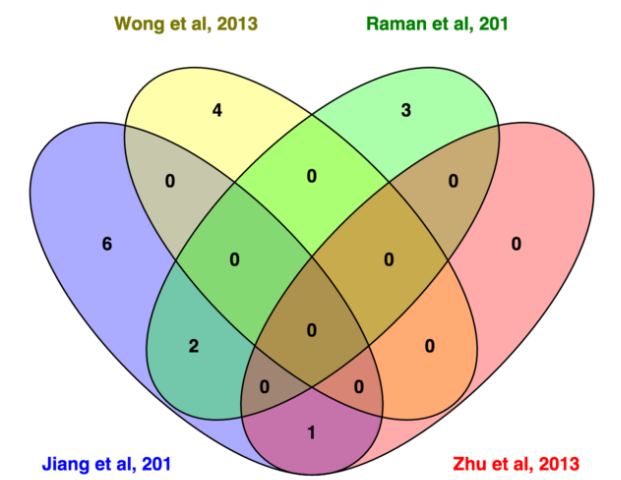
\includegraphics[width=0.7\textwidth]{nafld_papers.png}
\caption[Venn diagram of genera found to be differentially abundant by different studies between NASH/NAFLD and healthy controls.]{\textbf{Venn diagram of genera found to be differentially abundant by different studies between NASH/NAFLD and healthy controls.} Only 3 out of the 16 genera claimed to be differentially abundant were found in two studies: members of the \textit{Escherichia} genus were found in the Zhu \cite{zhu2013characterization} and Jiang \cite{jiang2015dysbiosis} studies, and members of the \textit{Lactobacillus} and \textit{Oscillibacter} genus were found in the Jiang \cite{jiang2015dysbiosis} and Raman \cite{raman2013fecal} studies. Of these, only Raman et al \cite{raman2013fecal} reported using a multiple test correction.}
\label{introduction_nafld_fig1}
\end{center}
\end{figure}

Fig. ~\ref{introduction_nafld_fig1} shows a Venn diagram illustrating the inconsistency of the literature on the gut microbiome and NAFLD. Of these, only Raman et al \cite{raman2013fecal} reported using a multiple test correction. Many of the studies had healthy controls with a lower BMI, so it is difficult to separate whether the differences found are related to NAFLD progression or obesity. These five studies do not form a consistent story about the gut microbiome and NAFLD. In one chapter of this thesis, we conduct our own non alcoholic steatohepatosis gut microbiome study, such that our results are replicable. Additionally, we generate the first deeply sequenced metagenomic sample set to examine functional capabilities in this disease.

Our hypothesis for the gene tag sequencing experiment was that we would find significantly differentially abundant taxa. For the metagenomic experiment, we hypothesized that we would find significantly differential groups of gene functions.

We compare the gut microbiome of 29 patients with nonalcoholic steatohepatitis (NASH), 14 patients with simple steatosis (SS), and 24 healthy controls. We found no significantly differentially abundant features between groups. However, the effect sizes of OTUs between extreme and intermediate groups appear to be correlated with a subset of the samples selected with more stringent clinical criteria. We believe that there may be a real difference between patients, if a study were performed with sufficient power.